\scanpage{42}
Moyennant $C(Y)$, $C(X)$ équivaut à la condition
\[
\left|\begin{gathered}
\forall i\leq n-1,\quad\text{l'hom }\psi_\xi^i:H^i(Y)\longrightarrow H^i(X),\quad\text{inverse à gauche}\\
\text{naturel de }\varphi^i:H^i(X)\mathbin{-}H^i(Y),\quad\deleted{\text{et}}\quad\text{égal : }\Lambda_X\varphi_{i}\mid H^i(Y),\quad\text{est}\\
\text{induit par une classe algébrique.}
\end{gathered}\right.
\]
ou encore :
\[
\left|\quad\Lambda_X\varphi_*\text{ est algébrique}\right.
\]
\deleted{ou encore}\quad N.B. $\Lambda_X\varphi_*$ correspond à une classe de cohomologie
\inserted{$\text{dans }\sum H^{2(n-1)-i}(Y)\otimes H^i(X)=H^{2(n-2)}(X\times Y)=H^{m-1}(X\times Y),\ m=\dim X\times Y$}
sur $X\times Y$, que nous polarisons par $\xi_X\otimes1+1\otimes\xi_Y$.
Or \deleted{$\unsure{\xi_X\otimes1+}$} $L_{X\times Y}(\Lambda_X\varphi_*)$ correspond à
\[
\begin{aligned}
\underbrace{\Lambda_X\varphi_*L_Y}_{\Lambda_XL_X\varphi_*}
 +\underbrace{L_X\Lambda_X\varphi_*}
 &=\deleted{\left(2\operatorname{id}-\sum_{n\leq i\leq2n}p_i^X\right)\varphi_*}\\
 &\inserted{=(\Lambda_XL_X+L_X\Lambda_X)\varphi_*}\\
 &=(\varphi_*\Lambda_Y\varphi^*+\operatorname{id}_X)\varphi_*.
\end{aligned}
\]
\figure{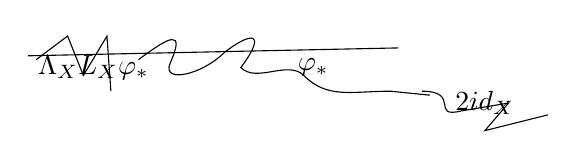
\begin{tikzpicture}[x=1cm,y=1cm]
\node[anchor=west] at (0,0) {$\deleted{\unsure{\Lambda_XL_X\varphi_*}}$};
\node[anchor=west] at (3.3,0) {$\deleted{\varphi_*}$};
\node[anchor=west] at (5.3,-.45) {$\deleted{\unsure{2\operatorname{id}_X}}$};
\draw (0,.15)--(4.7,.25);
\draw (.1,.1)--(.5,.4)--(.7,-.1)--(1,.4)--(1.05,-.3);
\draw (1.4,.1)..controls(1.8,.4)and(2,.5)..(1.8,.05)..controls(1.7,-.2)and(2.2,-.1)..(2.5,.2)..controls(2.9,.5)and(3,.4)..(2.7,.0)..controls(2.9,-.2)and(3.3,.1)..(3.5,-.1)..controls(3.8,-.4)and(4.1,-.3)..(4.6,-.3)--(5.1,-.35);
\draw (5.0,-.3)..controls(5.5,-.3)and(5.1,-.65)..(5.5,-.55)--(6.1,-.45)--(5.8,-.8)--(6.6,-.6);
\end{tikzpicture}}
(car $p_n^X\varphi_*=0$)

Donc est algébrique. Donc on trouve
\[
C(X)\Longleftrightarrow[C(Y)\text{ et }A^0(X\times Y)]
\]
puis de proche en proche
\[
C(X)\Longleftrightarrow\bigl(A^0(X\times Y)\text{ et }A^0(Y\times Z)\text{ et }A^0(Z\times T)\mathbin{-}\mathbin{-}\bigr)
\]
\deleted{$X\times Y,\ Y\times$}\quad
$X\supset Y\supset Z\supset T\mathbin{-}\mathbin{-}$ \unsure{pour une} suite décroissante de sections hyperplanes non singulières.

\figure{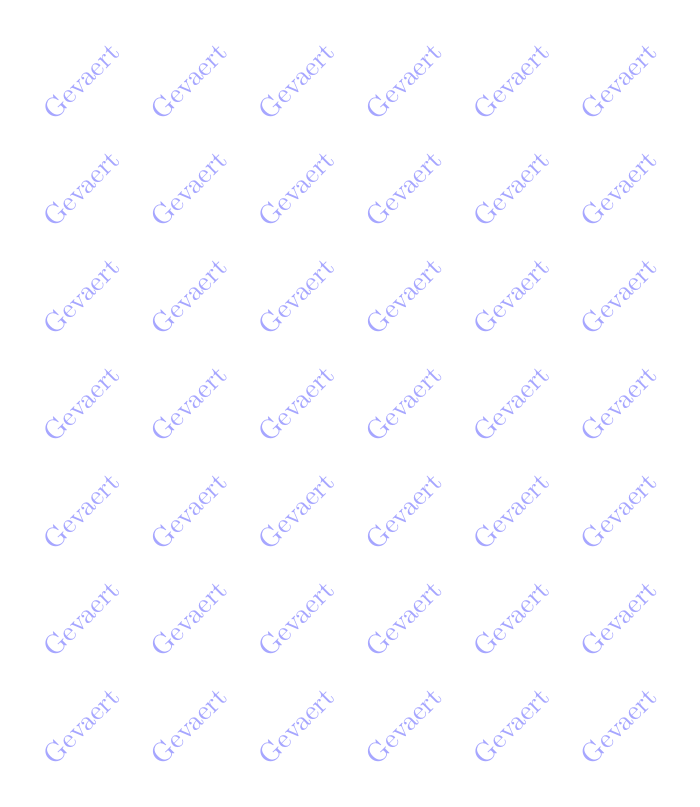
\begin{tikzpicture}[x=.65cm,y=.65cm]
\node[rotate=45,text=blue!35] at (0.0,12.600000000000001){Gevaert};
\node[rotate=45,text=blue!35] at (2.1,12.600000000000001){Gevaert};
\node[rotate=45,text=blue!35] at (4.2,12.600000000000001){Gevaert};
\node[rotate=45,text=blue!35] at (6.300000000000001,12.600000000000001){Gevaert};
\node[rotate=45,text=blue!35] at (8.4,12.600000000000001){Gevaert};
\node[rotate=45,text=blue!35] at (10.5,12.600000000000001){Gevaert};
\node[rotate=45,text=blue!35] at (0.0,10.5){Gevaert};
\node[rotate=45,text=blue!35] at (2.1,10.5){Gevaert};
\node[rotate=45,text=blue!35] at (4.2,10.5){Gevaert};
\node[rotate=45,text=blue!35] at (6.300000000000001,10.5){Gevaert};
\node[rotate=45,text=blue!35] at (8.4,10.5){Gevaert};
\node[rotate=45,text=blue!35] at (10.5,10.5){Gevaert};
\node[rotate=45,text=blue!35] at (0.0,8.4){Gevaert};
\node[rotate=45,text=blue!35] at (2.1,8.4){Gevaert};
\node[rotate=45,text=blue!35] at (4.2,8.4){Gevaert};
\node[rotate=45,text=blue!35] at (6.300000000000001,8.4){Gevaert};
\node[rotate=45,text=blue!35] at (8.4,8.4){Gevaert};
\node[rotate=45,text=blue!35] at (10.5,8.4){Gevaert};
\node[rotate=45,text=blue!35] at (0.0,6.300000000000001){Gevaert};
\node[rotate=45,text=blue!35] at (2.1,6.300000000000001){Gevaert};
\node[rotate=45,text=blue!35] at (4.2,6.300000000000001){Gevaert};
\node[rotate=45,text=blue!35] at (6.300000000000001,6.300000000000001){Gevaert};
\node[rotate=45,text=blue!35] at (8.4,6.300000000000001){Gevaert};
\node[rotate=45,text=blue!35] at (10.5,6.300000000000001){Gevaert};
\node[rotate=45,text=blue!35] at (0.0,4.2){Gevaert};
\node[rotate=45,text=blue!35] at (2.1,4.2){Gevaert};
\node[rotate=45,text=blue!35] at (4.2,4.2){Gevaert};
\node[rotate=45,text=blue!35] at (6.300000000000001,4.2){Gevaert};
\node[rotate=45,text=blue!35] at (8.4,4.2){Gevaert};
\node[rotate=45,text=blue!35] at (10.5,4.2){Gevaert};
\node[rotate=45,text=blue!35] at (0.0,2.1){Gevaert};
\node[rotate=45,text=blue!35] at (2.1,2.1){Gevaert};
\node[rotate=45,text=blue!35] at (4.2,2.1){Gevaert};
\node[rotate=45,text=blue!35] at (6.300000000000001,2.1){Gevaert};
\node[rotate=45,text=blue!35] at (8.4,2.1){Gevaert};
\node[rotate=45,text=blue!35] at (10.5,2.1){Gevaert};
\node[rotate=45,text=blue!35] at (0.0,0.0){Gevaert};
\node[rotate=45,text=blue!35] at (2.1,0.0){Gevaert};
\node[rotate=45,text=blue!35] at (4.2,0.0){Gevaert};
\node[rotate=45,text=blue!35] at (6.300000000000001,0.0){Gevaert};
\node[rotate=45,text=blue!35] at (8.4,0.0){Gevaert};
\node[rotate=45,text=blue!35] at (10.5,0.0){Gevaert};
\end{tikzpicture}}
\mspage{41}
